\subsection{Results}
\label{sec:tweets-attn-results}

The neural classifiers have an average accuracy of 73.9~\% and F$_1$ score of 72.5~\% across the ten initializations.%
\footnote{These scores cannot be directly compared to the classifier performances that \citet{chiril2020annotated} report for the same dataset, since their test set has a different label distribution than mine.
The test sets I work with all have a label ratio of approximately 1:2 (sexist content vs. non-sexist content), whereas \citeauthor{chiril2020annotated} use a more balanced ratio of circa 3:5.
That said, their neural, non-BERT models achieve accuracy scores of up to 69.5~\% and F$_1$ scores of up to 64.0~\%.
Their best model is a mulitilingual BERT model \citep{devlin2019bert} with a classification layer that has an accuracy of 79.0~\% and an F$_1$ score of 76.2~\%.}

I extract attention weights for tokens in the test sets and discard those that appear less than twenty times.
I then calculate the global attention score for each token by averaging the attention weights that the token is associated with in the different tweets and initializations.
The highest global attention score is 0.27.

I also examine the distribution of the attention weights per utterance.
On average, the entropy of the attention weight distribution for a tweet is 2.58, with a standard deviation of 1.24.
For comparison, the maximum possible entropy for a probability distribution with 60 possible outcomes is 4.09.
Some tweets have attention weight vectors that are very nearly one-hot encoded (with an entropy of 0.0001), i.e. where the attention lies very clearly on a single token, whereas some others have uniform attention distributions (with an entropy of 4.09), but most lie somewhere in the middle.

The {\ngram\filler} tokens have a mean attention weight of 0.01, i.e. an attention score that is only marginally higher than the weight of 0 one might expect.


\begin{figure}[htbp]
    \centering
    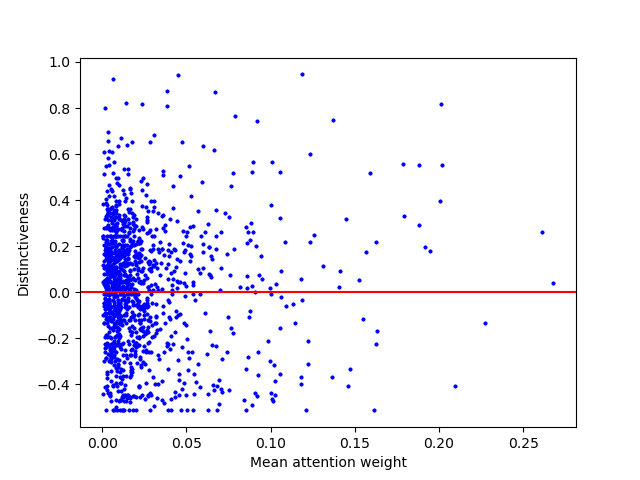
\includegraphics[width=0.9\textwidth]{figures/3-dialects/attention-distinctiveness.png}
    \caption[Distinctiveness values by attention weight for features in the Twitter data]{Distinctiveness values by global attention weight.}
    \label{fig:attn-dist}
\end{figure}

\autoref{fig:attn-dist} shows the global attention weights as well as the corresponding distinctiveness scores.
The latter are calculated with regard to the class of tweets with sexist content.
Positive distinctiveness scores indicate that a feature appears especially often in sexist tweets (the upper bound is 1.0) and negative scores indicate that a feature occurs especially often in non-sexist tweets (with a lower bound of -0.51).
Unlike in the LIME experiments, there is no significant correlation between the attention(/importance) score a feature has and how distinctive it is: many features that are very characteristic of one class of tweets have low attention weights, and some of the features with high global attention scores have distinctiveness values close to zero.
For instance, the feature with the highest attention score, \ngram{pourrait} `could,' has a distinctiveness score of only 0.04.

In the following section, I consider the 100 tokens with the highest global attention weights (this represents a range of attention scores from 0.08 to 0.27) and compare recurrent types of tokens present in that group to those present in the LIME results (\autoref{sec:tweets-svm-results}).
The full list of attention weights is available at \url{https://github.com/verenablaschke/ma-thesis/tree/main/models/tweets-attn}.

The attention weights are not label-specific---a high attention weight only means that the FFNN-encoded representation of a token receives a greater weight when making the final classification decision.
I therefore consider all (high-attention) features with positive distinctiveness scores to be indicators of sexist content, and features with negative distinctiveness scores to be important predictors for tweets with no sexist content.

% \subsection{Recurring feature types}

\subsubsection{Words relating to gender or sex}
\begin{table}[htbp]
    \centering
\begin{tabular}{llrrrl}
\toprule
\textbf{Group} & \textbf{Feature} & \multicolumn{1}{l}{\textbf{Imp.}} & \multicolumn{1}{l}{\textbf{Rep.}} & \multicolumn{1}{l}{\textbf{Dist.}} & \textbf{LIME?} \\
\midrule
\multirow{10}{*}{\begin{tabular}[c]{@{}l@{}}Sexist\\ content\end{tabular}} & \ngram{filles} `girls' & 0.20 & 0.02 & 0.55 &  \ngram{filles\eow}\\
 & \ngram{sexes} `sexes' & 0.20 & 0.01 & 0.39 &  \\
 & \ngram{femmes} `women' & 0.19 & 0.12 & 0.20 &  \ngram{femmes\eow}\\
 & \ngram{sexe} `sex' & 0.16 & 0.01 & 0.18 &  \\
 & \ngram{garçons} `boys'& 0.12 & 0.01 & 0.60 &  \\
 & \ngram{dame} `lady' & 0.10 & 0.00 & 0.02 & \\
 & \ngram{féminin} `feminine, female' & 0.09 & 0.01 & 0.07 & \\
 & \ngram{mecs} `guys' & 0.09 & 0.01 & 0.74 & \\
 & \ngram{fille} `girl' & 0.09 & 0.03 & 0.03 & \ngram{fille\eow}\\
 & \ngram{femme} `woman' & 0.09 & 0.23 & 0.26 & \ngram{femme\eow}\\
 \bottomrule
\end{tabular}
    \caption
    [Features with the top 100 highest attention scores relating to gender or sex]
    {Features with the top 100 highest attention scores relating to gender or sex.
    The middle columns contain importance, representativeness and distinctiveness\protect\footnotemark{} scores.
    The right-most column lists the corresponding features presented in \autoref{sec:tweets-svm-results}, if applicable.
    }
    \label{tab:attn-gender}
\end{table}
\footnotetext{Some of the distinctiveness scores deviate slightly from the corresponding ones in the LIME results due to the different tokenization approaches.}

Several of the words with high attention scores relate to gender or sex.
They are shown in \autoref{tab:attn-gender}.
Notably, all of these tend to occur especially often in tweets with sexist content (with the exception of \textit{dame} `lady,' which has a distinctiveness score that is barely above 0).
There is some overlap between this group and the gender-related words among the tokens with high LIME importance scores, but many of these terms appear only in the results of one experiment but not the other.
These differences \textit{cannot} be explained because of the vocabulary of the word2vec embeddings, since these also contain more colloquial terms like \textit{meuf} `woman' (which has a high LIME score).

\subsubsection{Words relating to feminism and sexism}
\begin{table}[htbp]
    \centering
\begin{tabular}{llrrrl}
\toprule
\textbf{Label} & \textbf{Feature} & {\textbf{Imp.}} & {\textbf{Rep.}} & {\textbf{Dist.}} & \textbf{Context} \\
\midrule
\multirow{4}{*}{\begin{tabular}[c]{@{}l@{}}Sexist\\ content\end{tabular}} & \ngram{féminisme\eow} & 0.11 & 0.01 & 0.30 & féminisme(1.0) `feminism' \\
 & \ngram{égalité\eow} & 0.08 & 0.03 & 0.40 & égalité(1.0) `equality'\\
 & \ngram{sexiste\eow} & 0.06 & 0.02 & 0.25 & sexiste(1.0) `sexist' \\
 & \ngram{féministe\eow} & 0.06 & 0.03 & 0.21 & féministe(1.0) `feminist'\\
 \midrule
\begin{tabular}[c]{@{}l@{}}No sexist\\ content\end{tabular} & \ngram{sexisme\eow} & 0.03 & 0.06 & 0.35 & sexisme(1.0) `sexism'\\
\bottomrule
\end{tabular}
    \caption
    [Features with the top 100 highest attention scores relating to feminism or sexism]
    {Features with the top 100 highest attention scores relating to feminism or sexism.
    The middle columns contain importance, representativeness and distinctiveness scores.
    The right-most column lists the corresponding features presented in \autoref{sec:tweets-svm-results}, if applicable.
    }
    \label{tab:attn-feminism}
\end{table}

As in the LIME results, many high-ranking words are directly related to feminism or sexism (\autoref{tab:attn-feminism}).
The corresponding features with high attention weights contain all of the feminism/sexism-related tokens with high LIME importance scores, as well as one additional term (\textit{parité} `parity').

\subsubsection{Gendered insults}

Three of the tokens with high attention weights are insults directed at women: \textit{connasse} `bitch' and \textit{salope} `slut, bitch' (both of which have (subtokens that have) high LIME importance scores for the class of sexist tweets) and \textit{pute} `whore' (which---unsurprisingly---almost exclusively appears in tweets with sexist content, but is not among the 50 features with the highest LIME importance scores for that class).

\subsubsection{Female politicians}
\begin{table}[htbp]
    \centering
\begin{tabular}{llrrrl}
\toprule
\textbf{Label} & \textbf{Feature} & \multicolumn{1}{l}{\textbf{Imp.}} & \multicolumn{1}{l}{\textbf{Rep.}} & \multicolumn{1}{l}{\textbf{Dist.}} & \textbf{Context} \\
\midrule
\multirow{9}{*}{\begin{tabular}[c]{@{}l@{}}No sexist\\ content\end{tabular}} & \ngram{Ségolène\eow} & 0.05 & 0.03 & 0.88 & Ségolène(1.0)  \\
 & \ngram{Christiane\eow} & 0.05 & 0.03 & 0.77 & Christiane(1.0)  \\
 & \ngram{Royal\eow} & 0.04 & 0.03 & 0.87 & Royal(1.0)  \\
 & \ngram{Angela\eow} & 0.03 & 0.06 & 0.86 & Angela(1.0)  \\
 & \ngram{Theresa\eow} & 0.03 & 0.03 & 0.91 & Theresa(1.0)  \\
 & \ngram{Christine\eow} & 0.03 & 0.02 & 0.77 & Christine(1.0)  \\
 & \ngram{Taubira\eow} & 0.03 & 0.03 & 0.74 & Taubira(1.0)  \\
 & \ngram{Lagarde\eow} & 0.02 & 0.01 & 0.78 & Lagarde(1.0)  \\
 & \ngram{May\eow} & 0.02 & 0.03 & 0.89 & May(1.0) \\
 \bottomrule
\end{tabular}
    \caption
    [Features with the top 100 highest attention scores relating to female politicians]
    {Features with the top 100 highest attention scores relating to female politicians.
    The middle columns contain importance, representativeness and distinctiveness scores.
    The right-most column lists the corresponding features presented in \autoref{sec:tweets-svm-results}, if applicable.
    }
    \label{tab:attn-politicians}
\end{table}

Similarly to the LIME results, several tokens with high attention scores refer to female politicians.
There is only partial overlap between the two experiments' results however, and the attention-based results also include (female) job titles in addition to names of politicians (\autoref{tab:attn-gender}).
With the exception of the last name of Marlène Schiappa (who used to be the French Secretary of State for Gender Equality), all of these tokens mostly appear in tweets without sexist content. 

\subsubsection{Pronouns and punctuation}

Unlike the results of the LIME experiment, none of the high-ranking tokens are personal pronouns or contain punctuation marks.

\subsubsection{Body parts}
\begin{table}[htbp]
    \centering
\begin{tabular}{llrrrl}
\toprule
\textbf{Group} & \textbf{Feature} & \multicolumn{1}{l}{\textbf{Imp.}} & \multicolumn{1}{l}{\textbf{Rep.}} & \multicolumn{1}{l}{\textbf{Dist.}} & \textbf{LIME?} \\
\midrule
\multirow{3}{*}{\begin{tabular}[c]{@{}l@{}}Sexist\\ content\end{tabular}} & \ngram{seins} `breasts' & 0.20 & 0.01 & 0.82 &  \\
 & \ngram{bite} `dick' & 0.14 & 0.01 & 0.75 &  \\
 & \ngram{fesses} `buttocks' & 0.08 & 0.01 & 0.77 & \\
 \bottomrule
\end{tabular}
    \caption
    [Features with the top 100 highest attention scores describing body parts]
    {Features with the top 100 highest attention scores describing body parts.
    The middle columns contain importance, representativeness and distinctiveness scores.
    The right-most column lists the corresponding features presented in \autoref{sec:tweets-svm-results}, if applicable.
    }
    \label{tab:attn-body}
\end{table}

Three of the tokens with high global attention weights refer to body parts, as shown in \autoref{tab:attn-body}.
All of these words mostly appear in tweets with sexist content, and none of them are among the tokens with the highest LIME importance scores.
